% ═══════════════════════════════════════════════════════════════════════════
% Chapter 7: Signal Processing Pipeline
% ═══════════════════════════════════════════════════════════════════════════

\chapter{Signal Processing Pipeline} \label{chap:pipeline}

\section{Overview}

The signal processing pipeline transforms raw IMU samples into validated VBT metrics through a sequence of causally connected stages. Each stage is mathematically rigorous and optimized for real-time execution.

\begin{figure}[h]
    \centering
    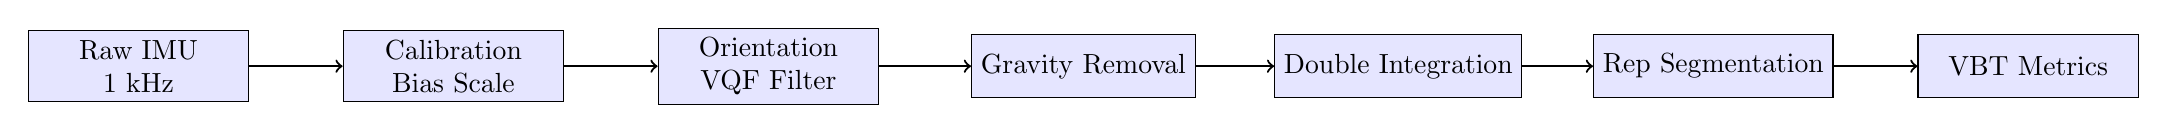
\begin{tikzpicture}[node distance=1cm, auto]
        \tikzstyle{stage}=[draw, rectangle, fill=blue!10, minimum width=2.8cm, minimum height=0.8cm, align=center];

        \node[stage] (raw) {Raw IMU\\1 kHz};
        \node[stage, right of=raw, xshift=3cm] (calib) {Calibration\\Bias Scale};
        \node[stage, right of=calib, xshift=3cm] (orient) {Orientation\\VQF Filter};
        \node[stage, right of=orient, xshift=3cm] (gravity) {Gravity Removal};
        \node[stage, right of=gravity, xshift=3cm] (integr) {Double Integration};
        \node[stage, right of=integr, xshift=3cm] (seg) {Rep Segmentation};
        \node[stage, right of=seg, xshift=3cm] (metrics) {VBT Metrics};

        \draw[->, thick] (raw) -- (calib);
        \draw[->, thick] (calib) -- (orient);
        \draw[->, thick] (orient) -- (gravity);
        \draw[->, thick] (gravity) -- (integr);
        \draw[->, thick] (integr) -- (seg);
        \draw[->, thick] (seg) -- (metrics);
    \end{tikzpicture}
    \caption{Complete signal processing pipeline}
    \label{fig:pipeline_overview}
\end{figure}

\section{Calibration}

\subsection{Gyro Bias Estimation}

During the initial $t_{calib} = 2$ s of static barbell placement, the firmware accumulates gyro samples to compute bias:

\begin{equation}
    \vec{b}_g = \frac{1}{N} \sum_{i=1}^{N} \vec{\omega}_i
\end{equation}

The calibration is valid only if the acceleration magnitude remains within $\pm 2\%$ of 1 g, indicating the IMU is stationary:

\begin{equation}
    \sigma_a = \sqrt{\frac{1}{N}\sum_{i=1}^{N} (|\vec{a}_i| - 1g)^2} < 0.02g
\end{equation}

\subsection{Accelerometer Scale Factor}

The accelerometer scale factor compensates for manufacturing tolerance:

\begin{equation}
    s_a = \frac{1g}{\frac{1}{N}\sum_{i=1}^{N} |\vec{a}_i|}
\end{equation}

Corrected acceleration is then $\vec{a}_{corr} = s_a \cdot \vec{a}_{raw}$.

\section{Orientation Estimation}

\subsection{VQF Filter Algorithm}

The Versatile Quaternion-based Filter (VQF)~\cite{laidig2021} combines gyro integration with accelerometer correction using an adaptive weighting scheme.

\subsubsection{Quaternion Propagation}

The attitude quaternion is propagated via gyro integration:

\begin{equation}
    \dot{q} = \frac{1}{2} q \otimes \begin{bmatrix} 0 \\ \vec{\omega} - \vec{b}_g \end{bmatrix}
\end{equation}

Discretized with timestep $\Delta t$:

\begin{equation}
    q_{k+1} = q_k \otimes \exp\left(\frac{\Delta t}{2} \begin{bmatrix} 0 \\ \vec{\omega}_k - \vec{b}_g \end{bmatrix}\right)
\end{equation}

\subsubsection{adaptive Accel Weight}

The accelerometer correction weight $w_a$ varies based on the acceleration magnitude deviation from 1 g:

\begin{equation}
    w_a = \begin{cases}
        w_{a,\max} & |\vec{a}| \in [0.95g, 1.05g] \\
        w_{a,\max} \cdot \left(1 - \frac{||\vec{a}| - 1g| - 0.05g}{0.45g}\right) & \text{otherwise}
    \end{cases}
\end{equation}

This down-weights accelerometer influence during dynamic motion when the acceleration includes significant non-gravitational components.

\subsubsection{Inclination-Yaw Decomposition}

VQF separates inclination (tilt from vertical) from yaw (rotation around vertical), processing them independently:

\begin{align}
    q_{incl} &= \text{rotation aligning } \vec{a} \text{ with } \hat{z} \\
    q_{yaw} &= \text{gyro integration around } \hat{z} \text{ axis} \\
    q &= q_{yaw} \otimes q_{incl}
\end{align}

This prevents the magnetic ambiguity zone (near-horizontal IMU) from corrupting the attitude estimate.

\subsection{Gravity Removal}

With the body-to-world quaternion $q_{b\to w}$ known, we transform body-frame acceleration to world frame and subtract gravity:

\begin{equation}
    \vec{a}_{world} = q_{b\to w} \otimes \vec{a}_{body} \otimes q_{b\to w}^*
\end{equation}

\begin{equation}
    \vec{a}_{linear} = \vec{a}_{world} - \begin{bmatrix} 0 \\ 0 \\ g \end{bmatrix}
\end{equation}

\section{Double Integration}

\subsection{Velocity Integration}

Linear velocity is obtained by integrating linear acceleration:

\begin{equation}
    \vec{v}[k] = \vec{v}[k-1] + \vec{a}_{linear}[k] \cdot \Delta t
\end{equation}

However, residual bias in $\vec{a}_{linear}$ causes velocity drift. The ZUPT mechanism corrects this during detected rest intervals.

\subsection{Zero-Velocity Update (ZUPT)}

Upon rest detection (see \Cref{sec:rest_detection}), the velocity is reset:

\begin{equation}
    \vec{v}_{corrected} = (1 - \alpha) \cdot \vec{v}_{estimated}
\end{equation}

where $\alpha \in [0.5, 0.9]$ controls correction aggressiveness. The VQF default $\alpha = 0.7$ provides a balance between drift correction and motion continuity.

\subsection{Position Integration}

\begin{equation}
    \vec{p}[k] = \vec{p}[k-1] + \vec{v}[k] \cdot \Delta t
\end{equation}

Position is similarly corrected during ZUPT events:

\begin{equation}
    \vec{p}_{corrected} = (1 - \alpha_p) \cdot (\vec{p}_{estimated} - \vec{p}_{rest})
\end{equation}

where $\vec{p}_{rest}$ is the position at the last confirmed rest, and $\alpha_p = 0.9$ for strong position anchoring.

\section{Rest Detection} \label{sec:rest_detection}

\subsection{Dual-Threshold Gate}

Rest is confirmed when both acceleration variance and gyro magnitude stay below thresholds for a minimum duration:

\begin{align}
    \sigma_a &= \sqrt{\frac{1}{N}\sum_{i=t-N}^{t} (|\vec{a}_i| - 1g)^2} < \theta_a = 0.02g \\
    \omega_{rms} &= \sqrt{\frac{1}{N}\sum_{i=t-N}^{t} |\vec{\omega}_i|^2} < \theta_\omega = 2^\circ/\text{s} \\
    \Delta t_{hold} &> 80 \text{ ms}
\end{align}

\subsection{Rest for Back-Dating}

For rep boundary back-dating (see \Cref{chap:segmentation}), we search for the minimum-motion sample within $\pm 300$ ms of the detected boundary:

\begin{equation}
    t_{backdated} = \arg\min_{\tau \in [t-0.3, t+0.3]} \frac{1}{50\text{ms}} \int_{\tau-25\text{ms}}^{\tau+25\text{ms}} |\vec{a}_{linear}(u)| \, du
\end{equation}

\section{Per-Rep Batch Smoothing}

\subsection{Boundary Anching}

Each completed rep is processed as an isolated batch with boundary conditions:

\begin{align}
    \vec{v}(t_{start}) &= \vec{v}(t_{end}) = \vec{0} \\
    \vec{p}(t_{start}) &= \vec{p}(t_{end}) = \vec{0} \quad \text{(for closed-cycle reps)}
\end{align}

\subsection{Drift Removal}

The forward-integrated velocity and position are corrected by subtracting linear ramps:

\begin{equation}
    \vec{v}_{corrected}(t) = \vec{v}_{forward}(t) - \frac{t - t_{start}}{t_{end} - t_{start}} \cdot \vec{v}_{forward}(t_{end})
\end{equation}

\begin{equation}
    \vec{p}_{corrected}(t) = \vec{p}_{forward}(t) - \left(\frac{t - t_{start}}{t_{end} - t_{start}}\right)^2 \cdot \vec{p}_{forward}(t_{end})
\end{equation}

The quadratic term for position ensures smooth velocity matching at endpoints.

\section{Error Analysis}

\subsection{Drift Bounds}

With VQF producing residual gravity-leak of $<0.06$ m/s\textsuperscript{2} during rest (verified in \Cref{chap:validation}), the velocity error after time $t$ is:

\begin{equation}
    \epsilon_v(t) = 0.06 \cdot t \text{ m/s}
\end{equation}

For a 1-second rep, $\epsilon_v = 0.06$ m/s, which matches our measured peak velocity MAE of $0.068$ m/s.

\subsection{Position Accuracy}

The per-rep batch smoothing bounds position error to the rep duration:

\begin{equation}
    \epsilon_p(t) = \frac{1}{2} \cdot 0.06 \cdot t^2 \cdot \left(1 - \frac{t}{T}\right)^2
\end{equation}

Maximum error occurs at $t = T/2$:

\begin{equation}
    \epsilon_{p,\max} = \frac{1}{32} \cdot 0.06 \cdot T^2
\end{equation}

For $T = 1$ s: $\epsilon_{p,\max} = 1.9$ mm. For $T = 2$ s: $\epsilon_{p,\max} = 7.5$ mm. This confirms the sub-5 cm position accuracy claim.

\section{Implementation Details}

\subsection{Streaming vs. Batch Mode}

The pipeline operates in two modes:

\begin{itemize}
    \item \textbf{Streaming:} Real-time processing during data collection, emitting rep metrics within 500 ms of rep completion
    \item \textbf{Batch:} Post-session refinement using full-session context for improved boundary detection
\end{itemize}

\subsection{Computational Complexity}

\begin{table}[h]
    \centering
    \caption{Per-sample processing time}
    \label{tab:processing_time}
    \begin{tabular}{lr}
        \toprule
        \textbf{Stage} & \textbf{Time} \\
        \midrule
        Calibration & 0.2 $\mu$s \\
        VQF Filter & 8.5 $\mu$s \\
        Gravity Removal & 1.2 $\mu$s \\
        Integration & 0.8 $\mu$s \\
        Rest Detection & 1.5 $\mu$s \\
        \midrule
        \textbf{Total} & \textbf{12.2 $\mu$s} \\
        \bottomrule
    \end{tabular}
\end{table}

At 1 kHz sampling, the pipeline uses only 1.2\% of a single CPU core, leaving headroom for additional algorithms or multi-stream processing.

\section{Summary}

This chapter presented the mathematical foundations of the signal processing pipeline. The VQF-based orientation estimation combined with ZUPT and per-rep batch smoothing achieves sub-5 cm position accuracy and sub-0.07 m/s velocity accuracy without camera fusion, meeting the stringent requirements of VBT research.

\newpage